\chapter{Introduction}

%第一段：介绍背景：电子商务带来多个挑战，第一个是更高的存储容量。但是在城市地区，土地稀缺和高昂的成本限制了简单扩建仓库以满足需求的可行性。因此，提高存储密度成为更可行的解决方案。
In recent years, e-commerce has maintained rapid growth worldwide. According to the global Business-to-Consumer (B2C) e-commerce forecast report published by ResearchAndMarkets, the global B2C e-commerce market achieved a compound annual growth rate (CAGR) of 9.5\% during 2020--2024. The report further forecasts continued growth over 2025--2029, with the market forecast to increase from USD 7.25 trillion in 2025 to approximately USD 9.21 trillion by 2029, corresponding to a CAGR of 6.2\% \cite{ResearchAndMarkets2025}. This growth has also brought multifaceted challenges to warehousing systems. One significant challenge is that e-commerce-driven order growth increases the demand for storage capacity. However, in metropolitan areas, the scarcity and high cost of land limit the feasibility of simply expanding warehouses to meet this demand \cite{Xiao2021,Sakai2024}. Consequently, for warehouses with limited expansion potential, increasing storage density is a more viable solution.

%第二段：引入多深位布局，先介绍多深位布局带来的存储密度提升，再介绍多深位布局引入的复杂取货逻辑（尤其是relocation问题）和效率下降问题。二者之间存在权衡关系。
Multi-deep storage layouts are one common approach for increasing storage density. Compared with traditional single-deep layouts, multi-deep layouts improve floor-space utilization by reducing the proportion of aisle space. With the increasing adoption of automated warehousing systems in recent years, multi-deep layouts have also been incorporated into automated vehicle storage and retrieval systems (AVS/RSs), offering a compact storage solution with high space utilization. However, multi-deep layouts also introduce more complex retrieval logic. If a target item is located deeper in a storage lane and is blocked by other non-target items, the target item can only be retrieved after all blocking non-target items have been moved to empty storage locations (in this paper, we denote this process as “relocation”). Each relocation process involves additional time, which negatively affects the operational efficiency of the system \cite{Marolt2022}. Fig. \ref{fig:layout} illustrates the structural differences between single-deep and multi-deep layouts and highlights the trade-off between space utilization and operational efficiency in multi-deep layouts.
\begin{figure}[htbp]
\centering
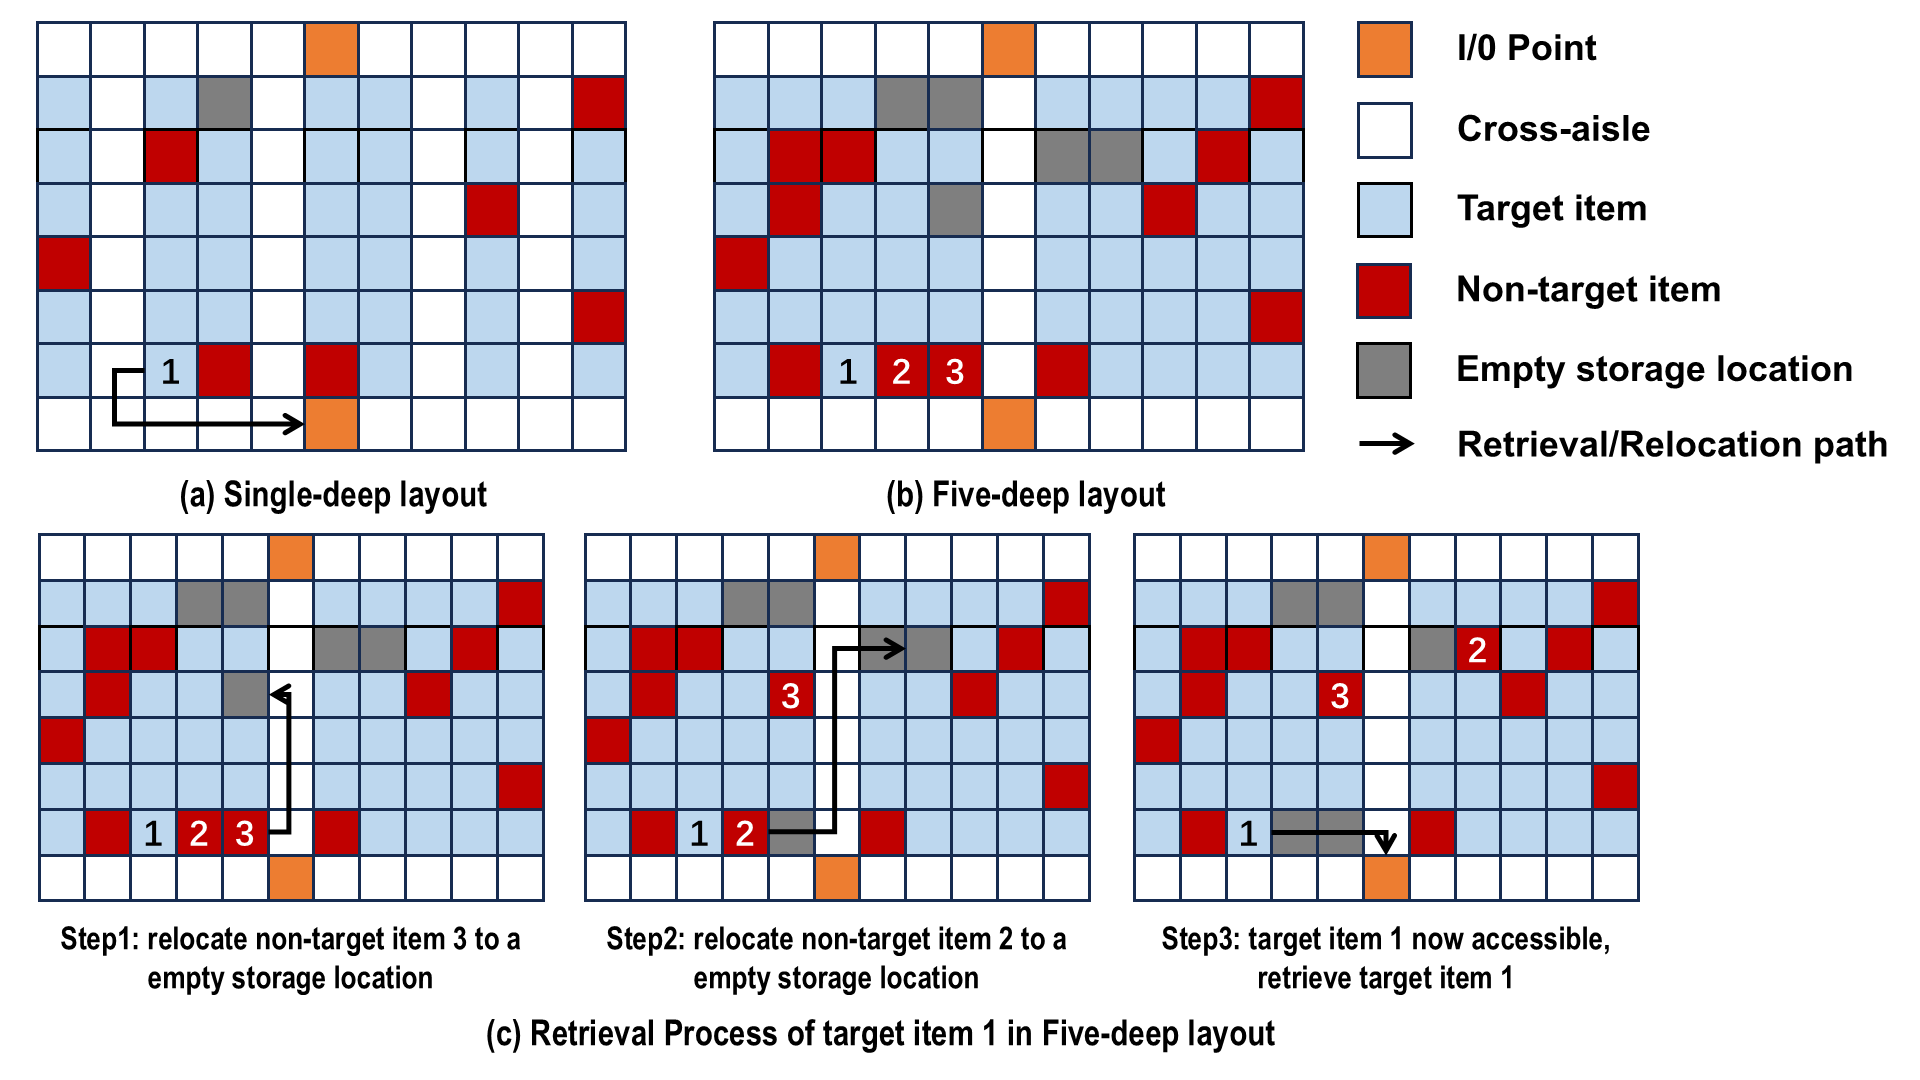
\includegraphics[width=\textwidth]{graphics/fig1.png}
\caption{Comparison of single-deep and five-deep layouts in terms of space utilization and operational efficiency}
\label{fig:layout}
\end{figure}
%第三段：介绍由电子商务带来的第二个挑战：当日达服务的普及提高了客户对交货速度和交货时间可靠性的期望，使客户对订单迟到更敏感。这给仓储系统带来了更大的履行压力，并对运营效率提出了更高的要求。*同时！*在多深位布局中，由于更复杂的取货逻辑导致的取货效率降低进一步增加了最小化总迟到时间的难度。
Another significant challenge stems from the widespread adoption of same-day and next-day delivery services driven by e-commerce. Amazon reported that, in 2025, more than 13 billion items were delivered to Prime members worldwide on the same day or the next day; among them, more than 8 billion items were delivered to Prime members in the United States on the same day or the next day, representing an increase of more than 30\% over the previous year \cite{Amazon2026}. The widespread adoption of such services has raised consumer expectations for delivery speed and delivery-time reliability, making customers more sensitive to late deliveries \cite{Ahmed2024,Paluzzi2025}. From a scheduling perspective, this makes tardiness-related performance increasingly important and places greater fulfillment pressure on warehousing systems. In multi-deep layouts, additional retrieval time caused by relocation further increases the complexity of tardiness-oriented scheduling processes.

%第四段：当前许多研究是启发式或元启发式方法-有缺点问题。 关于当前文献引用：2023年以来多深位仓库的调度问题（另有其他一些文章研究多深位仓库的建模仿真等问题）一共找到了5篇（不包括Li 2026）,其中三篇为启发式/元启发式，两篇为DRL方法。因此额外引用了一篇2021年的启发式方法文章。
Against this background, several recent studies have investigated scheduling problems in multi-deep warehousing systems. Many of these studies employ heuristic approaches \cite{Dong2021,Yang2023} or metaheuristic approaches \cite{Ren2025,Liu2026}. Although these approaches can produce high-quality solutions for their target problem settings, their performance often relies on problem-specific rules, neighborhood structures, or search operators. When warehouse layouts, task distributions, or operational constraints differ substantially from the setting assumed in the studies, these approaches may require redesign, recalibration, or repeated instance-specific optimization. Therefore, developing scheduling strategies with stronger adaptability and generalizability remains an important research issue in multi-deep warehousing systems.

%第五段：介绍DRL(RL引用Sutton2018，DRL引用Mnih2015)以及其近两年在复杂决策问题的应用（此处引用研究都为调度问题的应用），随后综述了DRL在高密度仓库（He2023的研究属于puzzle based不算multi deep）调度问题上的两篇相关研究。 *问题*：Xu2026的研究能否同时出现在此处的简单综述与后续的gap描述上？？？
In response to this research issue, the rapid development of machine learning (ML) in recent years has provided a new perspective. As an important subfield of ML, reinforcement learning (RL) optimizes a decision strategy through interactions with the environment and reward feedback \cite{SuttonBarto2018}; when combined with deep neural networks (DNNs), deep reinforcement learning (DRL) further improves the ability to learn effective representations from high-dimensional state inputs \cite{Mnih2015}. Scheduling problems have become an important application domain of DRL, and related studies have covered various complex scenarios, including dynamic task scheduling in stochastic edge--cloud computing environments \cite{Lu2024}, large-scale task scheduling for multiple unmanned aerial vehicles (UAVs) \cite{Mao2025}, and dynamic job-shop scheduling under processing-time uncertainty \cite{Wu2024}. These studies indicate that DRL can learn effective scheduling strategies in complex dynamic environments and improve real-time decision-making capability. The application of DRL to complex scheduling problems has also driven its adoption in high-density warehousing systems. He et al. adopted a Double \& Dueling Deep Q-Network to solve the multi-item retrieval problem in a puzzle-based storage system and demonstrated its superior performance over conventional heuristic strategies \cite{He2023}. Xu et al. employed a Deep Q-Network to address the real-time transaction scheduling problem in a multi-deep tier-to-tier shuttle-based storage and retrieval system (MDT-SBS/RS), outperforming several classical scheduling strategies under different system configurations \cite{Xu2026}.

%第六段：定位当前研究空白：很多高密度（此处使用高密度是为了引用研究puzzle based的He2023）仓库调度研究是静态调度问题（此处引用了上面的四篇启发式研究+He2023的puzzle based）。Li2025的研究(*问题*：后续是否需要更新为Li2026的研究？？？)与本文最相关，但仍然是一个静态调度问题，没有动态到达过程也没有重定位过程。虽然Xu2026等人考虑了动态随机订单到达，但他们的优化目标是平均周期时间，而不是总迟到时间，并且仓库中的物品没有建模为具有个体截止日期。
Despite recent progress in scheduling for high-density warehouse systems, most existing studies assume that retrieval requests or target items are known before scheduling starts \cite{Dong2021,Yang2023,He2023,Ren2025,Liu2026}. The study by Li et al. \cite{Li2025} is the most closely related to the problem investigated in this paper, as it also focuses on the retrieval scheduling problem in multi-deep AVS/RSs with the objective of minimizing total tardiness. However, their problem setting assumes a predefined initial target item set: in the initial state, the warehouse is fully occupied by the target items with known individual due dates. In contrast, in real warehouse environments, orders are usually not fully known in advance, but may arrive dynamically and stochastically during the scheduling process. Therefore, it is more realistic for the warehouse to contain non-target items in its initial state. Each arriving order activates one or more initially non-target items and assigns them due dates. Such initially non-target items may be located at different storage depths. They may currently block other target items, but may also be activated by future orders and subsequently become blocked by other items. This dynamic target-item activation mechanism couples retrieval and relocation processes over time and substantially increases the complexity of total tardiness minimization. One exception is Xu et al. \cite{Xu2026}, who consider stochastic order arrivals in real-time transaction scheduling. However, their optimization objective is the average cycle time rather than total tardiness, and items in the warehouse are not modeled with individual due dates.

%第七段：本文任务描述+问题难度定位+贡献总结
Motivated by this gap, this paper investigates the retrieval and relocation scheduling problem in multi-deep AVS/RSs with dynamic order-driven target-item activation, with the objective of minimizing total tardiness. Specifically, this paper extends a graph-based hierarchical DRL framework to this dynamic environment and designs a novel tardiness-oriented reward function to guide the learned strategy toward total tardiness minimization. This problem can be viewed as a dynamic and tardiness-oriented generalization of the classic Block Relocation Problem (BRP), which has been shown to be NP-hard \cite{Caserta2012}. Unlike the classic BRP, which is typically defined over a static set of blocks, the problem studied here requires coordinated retrieval and relocation decisions under dynamic order-driven target-item activation and individual due-date constraints. Since non-target items may both block currently active target items and later become new target items with due dates, the dynamic evolution of the target item set further increases the combinatorial complexity of the problem. The main contributions of this paper are fourfold:

\begin{enumerate}
    \item This paper considers a more realistic multi-deep AVS/RS environment with a dynamic order-arrival mechanism. In this environment, initially non-target items can be dynamically and stochastically activated as new target items during operation and assigned due dates, which better reflects real-world warehouse environments where orders arrive over time. This setting requires coordinated retrieval and relocation decisions, which makes the scheduling problem more relevant to real-world order-fulfillment scenarios.

    \item This paper designs a tardiness-oriented reward mechanism. A global incremental tardiness penalty is used to capture the increase in tardiness of all currently active target items, and a buffered tardiness mechanism based on static shortest-path distances is designed to reflect potential tardiness risks in the reward signal.

    \item This paper extends a graph-based hierarchical DRLdeep reinforcement learning framework of Li et al. \cite{Li2025} to the dynamic multi-deep AVS/RS environment, and integrates Graph Attention Network (GAT)-based encoders to model local topology, blocking relationships, and urgency differences among target items more flexibly.
    
    \item  numerical experiments (to be finished)
\end{enumerate}